\documentclass[11pt]{article}
\usepackage[utf8]{inputenc}
\usepackage{amsfonts, amssymb, amsmath}
\usepackage{fullpage}
\usepackage{float}
\usepackage{wrapfig}
\usepackage{natbib}
\usepackage{graphicx}
\usepackage[margin=2cm]{caption}
\usepackage{cancel}
\usepackage{tcolorbox}
\usepackage[shortlabels]{enumitem}
\usepackage{ wasysym }
\usepackage{caption}
\usepackage{subcaption}
\usepackage{tikz}
\usepackage{pgfplots}
\usetikzlibrary{arrows}
\input{longdiv}
\usepackage{longdivision}

\title{Multiple Choice Questions (Part 2 of 2)}
\author{Rafay A}
\date{19 December 2020}

\setlength{\parindent}{0in}

\newcommand{\choice}[1]{\textbf{(#1)}}


\def\fooA{
    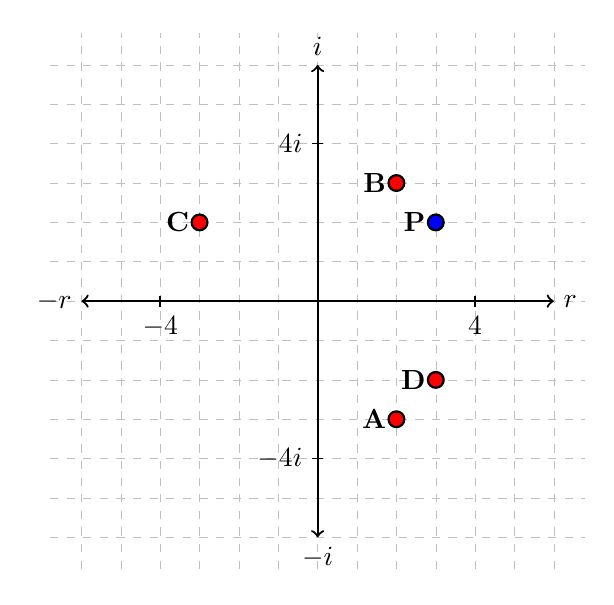
\begin{tikzpicture}
    % \fill [pink!50!white] (-3,-3) rectangle (3,3);
%    \draw[step=2cm,black,thin] (-2.9,-2.9) grid (2.9,2.9);
    \draw[step=.5cm,gray!50!white,very thin, dashed] (-3.4,-3.4) grid (3.4,3.4);
    \draw [thick, <->] (0,-3) -- (0,3);
    \draw [thick, <->] (-3,0) -- (3,0);
    \foreach \x in {-4,4}
	   \draw [thick](0.5*\x cm,2pt) -- (0.5*\x cm,-2pt) node[anchor=north] {$\x$};
	\foreach \y in {-4,4}
    	\draw (2pt,0.5*\y cm) -- (-2pt,0.5*\y cm) node[anchor=east] {$\y i$};
	\foreach \x/\y/\z in {2/-3/A,2/3/B,-3/2/C,3/-2/D}
	    	\draw [fill=red, thick] (0.5*\x,0.5*\y) circle (1mm) node[anchor= east] {\textbf{\z}};
%	    	\draw (0.5*\x, 0.5*\y) node[anchor=south] {$A$};
	\draw [fill= blue,thick](1.5,+1) circle (1mm) node[anchor=east] {\textbf{P}};
%	\draw [blue,thick, ->] (0,0) -- (1.5,-1);
    \draw (0,3) node[anchor = south] {$i$};
    \draw (3,0) node[anchor = west] {$r$};
    \draw (0,-3) node[anchor = north] {$-i$};
    \draw (-3,0) node[anchor = east] {$-r$};
%    \draw [red, thick,dashed, ->] (0,0) -- (30:2cm);
%    \draw [red, thick, ->] (0,0) -- (120:2cm);
%	\draw [blue!100!black,thick,->,domain=30:120] plot ({0.5*cos(\x)}, {0.5*sin(\x)});
%    \draw [blue!100!black] (0.3,0.5) node[anchor=south] {$90^{\circ}$};
    \end{tikzpicture}
}


\begin{document}
%------------------------------------------------
\begin{enumerate}[(1),wide,nosep, label={\bfseries \arabic*)}]
%------------------------------------------------
\item A cylinder of diameter 2 cm and circumference 2$\pi$ cm rolls along the number line. An arrow is painted on the cylinder. Initially, the arrow points straight down at 0, as shown in the figure below. As it rolls, the arrow rotates with it, and at point $3\pi$ the arrow points straight up, as shown in the figure.\\
At which point on the number line will the arrow point straight down once again?\\
\begin{figure}[H]
\centering
\begin{tikzpicture}[scale=1.5]
\draw[-latex] (-0.5,0) -- (8.5,0) node[right] {cm};
%\node[right] (8.5,0) {cm};
\foreach \x in {0,1,2,3,4,5,6,7,8}
	\draw[shift={(\x,0)},color=black] (0pt,3pt) -- (0pt,-3pt);
\foreach \x in {0,1,2,3,4,5,6,7}{
	\draw[shift={(\x+.50,0)},color=black] (0pt,2pt) -- (0pt,-2pt);
	\draw[shift={(\x+.25,0)},color=black] (0pt,1pt) -- (0pt,-1pt);
	\draw[shift={(\x+.75,0)},color=black] (0pt,1pt) -- (0pt,-1pt);
	}
\foreach \x in {0,1,2,3,4,5,6,7,8}
	\draw[shift={(\x,0)},color=black] (0pt,0pt) -- (0pt,-3pt) node[below] {$\x$};
\foreach \x/\y in {5.2/A,6.28/B,7.3/C,8/D}
	\draw [draw=red,thick, <-] (\x,0) -- (\x,3mm) node[above] {\y};
	
\draw[blue] (0,1) circle (1);
\draw[red,->,ultra thick] (0,0.8) -- (0,0.1);

\draw[blue, dashed] (3.143,1) circle (1);
\draw[red,->, ultra thick] (3.143,1.2) -- (3.143,1.9);
\draw[black,thick,domain=40:140,<-] plot ({1.1*cos(\x)}, {1.1+1.1*sin(\x)});
\draw[dashed,thick,->] (1.15,1.1) -- (1.85,1.1);
\draw[dashed,thick,->] (1.15,0.9) -- (1.85,0.9);

\end{tikzpicture}
\end{figure}

Correct Answer: \choice{B}\\
Each numbered interval is divided into four smaller interval. Hence, the smallest interval step is 0.25 units.\\
It is shown that at $\pi \approx 3.14$ cm, the arrow points straight up, hence the arrow will point straight down next, which will be at the point $2\pi \approx 2\times 3.14=6.28$, i.e. \choice B\\\\

Possible Mistakes:\\
- Choosing the closest value to 3 may lead to \choice D\\
- Incorrectly interpreting the negative value may lead to choosing \choice A or \choice B

\newpage

\item Which point shows the conjugate of the point P?
\begin{figure}[H]
\centering
\fooA
\end{figure}
\begin{tabular}{ll}
a)&\textbf{A}\\
b)&\textbf{B}\\
c)&\textbf{C}\\
d)&\textbf{D}\\
\end{tabular}\\\\

Correct Answer:  \choice d\\
The student may know that the conjugate of a complex number is its reflection about the $x$-axis, and locate \textbf{D} as the correct choice.\\\\
The student can also find the conjugate by first evaluating what is point \textbf{P}, i.e $3+2i$. Hence, the conjugate of this number will be $3-2i$, which is point \textbf{D}.\\\\

Possible Mistakes:\\
- A student may not remember whether to reflect \textbf{P} about the $x$-axis or $y$-axis and may incorrectly select \choice c\\
- A student may also flip the coordinates which may result in \choice b or \choice a

\newpage

%----------------------------------------------
\item How many factors would result from the complete factorization of $xy^2$?\\
\begin{tabular}{l}\\
    a) 1\\
    b) 2\\
    c) 3\\
    d) 4\\
\end{tabular}\\\\

Correct Answer: \choice c \\
The term $xy^2$ can be completely factorized as:
$$xy^2 = x \times y \times y$$
Hence, there are 3 factors \\\\

Possible Mistakes:\\
- The options are given an ordered form to emphasize there's no bias towards any option.\\
- \choice b can possibly be selected by factoring the expression into two terms as $x$ and $y^2$ 
\newpage
%------------------------------------------------
\item Identify the function for the given plot:
\begin{figure}[H]
	\centering
	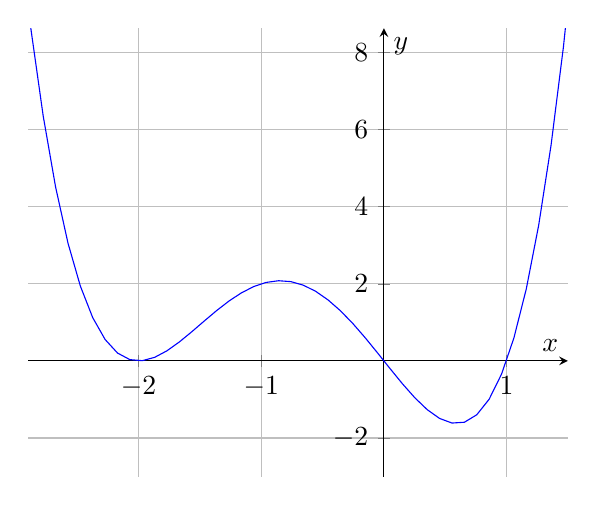
\begin{tikzpicture}
		\begin{axis}[samples=100, scale=1,
					ymin=-3,xmin=-2.9,xmax=1.5, 
					grid=both, xlabel=$x$, ylabel=$y$,
					axis lines = middle,
					minor tick num=0]
		\addplot[blue]{x*(x-1)*(x+2)^2};
		\end{axis}
	\end{tikzpicture}
\end{figure}
\begin{tabular}{ll}
a)&$f(x)=x(x+2)(x-1)$\\\\
b)&$f(x)=(x-1)(x+2)^2$\\\\
c)&$f(x)=x(x-1)(x+2)^2$\\\\
d)&$f(x)=(x-1)^2(x+1)^2$\\\\
\end{tabular}\\\\

Correct Answer: \choice c\\
The end conditions of the curve resembles that of $+x^{2n}$ where $n \in \mathbb{N}$ (i.e. even).\\
We're left with choices c and d, and both are degree 4 polynomials.\\
- The zeros can be identified from the plot as $x=-2$, $x=1$, and $x=0$.\\
- The multiplicity at $x=-2$ is 2.\\
- The equation can be written as: $(x+2)^2(x-1)x$\\
Hence the only choice with these conditions satisfied is choice \choice c\\\\

Possible Mistakes:\\
- Only focusing on the zeros of the plot may lead to \choice a\\
- Ignoring that the plot crosses the origin may lead to \choice b or \choice d\\
- Assuming odd degree of the polynomial may lead to \choice b

\newpage


\end{enumerate}
\end{document}